\documentclass[
	10pt,								% globale Schriftgröße
	parskip=half-,						% setzt Absatzabstand hoch
	paper=a4,							% Format
	english,ngerman,					% lädt Sprachpakete
	]{scrartcl}							% Dokumentenklasse

% //////////////////// Pakete laden ////////////////////
\usepackage{amsmath}			% MUSS vor fontspec geladen werden
\usepackage{mathtools}			% modifiziert amsmath
\usepackage{amssymb}			% mathematische symbole, für \ceckmarks
\usepackage{amsthm}				% für proof
\usepackage{mathrsfs}			% für \mathscr
\usepackage{latexsym}
\usepackage{marvosym}				% für Lightning

\usepackage{fontspec} 			% funktioniert nur mit den neueren Compilern z.B. XeLaTeX
\usepackage{microtype}			% für bessere Worttrennung
\usepackage[ngerman]{babel} 	% Spracheinstellung
\usepackage{csquotes}
\usepackage{lmodern}			% verändert verwendete Schriftart, damit sie weniger pixelig ist

\usepackage{verbatim}
\usepackage{listings}			% Für Quellcode

\usepackage{graphicx}
\usepackage{tabularx}			% für Tabellen mit gleicher Spaltenbreite und automatischen Umbrüchen
\usepackage{fullpage}
\usepackage{multirow}			% für multirow in tabulars
\usepackage{rotate}
\usepackage[cmyk,table]{xcolor} % um Farben zu benutzen, kann mehr als das Paket color
\usepackage[					% Verlinkungen
	colorlinks,					% farbige Schrift, statt farbiger Rahmen
	linktocpage,				% verlinkt im Abb.Verzeichnis Seitenzahl statt Bildunterschrift
	linkcolor=blue				% setzt Farbe der Links auf blau
	]{hyperref}					% nur für digitale Anwendungen, url = "http://www.example.com"
\usepackage{url}				% für Webadressen wie e-mail usw.: "\url{http://www.example.com}"

\usepackage{enumerate}			% für versch. Aufzählungezeichen wie z.B. a)
\usepackage{xspace}				% folgt ein Leerzeichen nach einem \Befehl, wird es nicht verschluckt.
\usepackage{cancel}				% für das Durchstreichen u.a. in Matheformeln mit \cancel
\usepackage{float}              % zum Forcieren der Position von figure-Umgebungen

% zum Zeichnen (u.a. von Graphen)
\usepackage{fp}
\usepackage{tikz}
\usetikzlibrary{tikzmark}			% für \tikzmark{toRemember}
\usetikzlibrary{positioning}	% verbesserte Positionierung der Knoten
\usetikzlibrary{automata}		% für Automaten (GTI)
\usetikzlibrary{arrows}
\usetikzlibrary{shapes}
\usetikzlibrary{decorations.pathmorphing}
\usetikzlibrary{decorations.pathreplacing}
\usetikzlibrary{decorations.shapes}
\usetikzlibrary{decorations.text}

% //////////////////// Syntaxhighlighting ////////////////////
\lstloadlanguages{Python, Haskell, [LaTeX]TeX, Java}
\lstset{
   basicstyle=\footnotesize\ttfamily,	% \scriptsize the size of the fonts that are used for the code
   backgroundcolor = \color{bgcolour},	% legt Farbe der Box fest
   breakatwhitespace=false,	% sets if automatic breaks should only happen at whitespace
   breaklines=true,			% sets automatic line breaking
   captionpos=t,				% sets the caption-position to bottom, t for top
   commentstyle=\color{codeblue}\ttfamily,% comment style
   frame=single,				% adds a frame around the code
   keepspaces=true,			% keeps spaces in text, useful for keeping indentation
							% of code (possibly needs columns=flexible)
   keywordstyle=\bfseries\ttfamily\color{codepurple},% keyword style
   numbers=left,				% where to put the line-numbers;
   							% possible values are (none, left, right)
   numberstyle=\tiny\color{codegreen},	% the style that is used for the line-numbers
   numbersep=5pt,			% how far the line-numbers are from the code
   stepnumber=1,				% nummeriert nur jede i-te Zeile
   showspaces=false,			% show spaces everywhere adding particular underscores;
							% it overrides 'showstringspaces'
   showstringspaces=false,	% underline spaces within strings only
   showtabs=false,			% show tabs within strings adding particular underscores
   flexiblecolumns=false,
   tabsize=1,				% the step between two line-numbers. If 1: each line will be numbered
   stringstyle=\color{orange}\ttfamily,	% string literal style
   numberblanklines=false,				% leere Zeilen werden nicht mitnummeriert
   xleftmargin=1.2em,					% Abstand zum linken Layoutrand
   xrightmargin=0.4em,					% Abstand zum rechten Layoutrand
   aboveskip=2ex, 
}

\lstdefinestyle{py}{
   language=Python,
}
\lstdefinestyle{hs}{
   language=Haskell,
}
\lstdefinestyle{tex}{
	language=[LaTeX]TeX,
	escapeinside={\%*}{*)},     % if you want to add LaTeX within your code
	texcsstyle=*\bfseries\color{blue},% hervorhebung der tex-Schlüsselwörter
	morekeywords={*,$,\{,\},\[,\],lstinputlisting,includegraphics,
	rowcolor,columncolor,listoffigures,lstlistoflistings,
	subsection,subsubsection,textcolor,tableofcontents,colorbox,
	fcolorbox,definecolor,cellcolor,url,linktocpage,subtitle,
	subject,maketitle,usetikzlibrary,node,path,addbibresource,
	printbibliography},% if you want to add more keywords to the set
     numbers=none,
     numbersep=0pt,
     xleftmargin=0.4em,
}

\lstdefinestyle{java}{
	language=Java,
	extendedchars=true,		% lets you use non-ASCII characters;
   						% for 8-bits encodings only, does not work with UTF-8
}

\lstdefinelanguage[x64]{Assembler}     % add a "x64" dialect of Assembler
   [x86masm]{Assembler} % based on the "x86masm" dialect
   % with these extra keywords:
   {morekeywords={CDQE,CQO,CMPSQ,CMPXCHG16B,JRCXZ,LODSQ,MOVSXD, %
                  POPFQ,PUSHFQ,SCASQ,STOSQ,IRETQ,RDTSCP,SWAPGS, %
                  rax,rdx,rcx,rbx,rsi,rdi,rsp,rbp, %
                  r8,r8d,r8w,r8b,r9,r9d,r9w,r9b}
}					% for 8-bits encodings only, does not work with UTF-8

\lstdefinestyle{c}{
	language=c,
	extendedchars=true,		% for 8-bits encodings only, does not work with UTF-8
}

% //////////////////// eigene Kommandos ////////////////////
\newcommand\FU{Freie Universität Berlin\xspace}% benötigt package xspace
\newcommand\gdw{g.\,d.\,w.\xspace}
\newcommand\oBdA{o.\,B.\,d.\,A.\xspace}
\newcommand{\Eu}{\texteuro}
\newcommand\N{\mathbb{N}\xspace}
\newcommand\Q{\mathbb{Q}\xspace}
\newcommand\R{\mathbb{R}\xspace}
\newcommand\Z{\mathbb{Z}\xspace}
\newcommand\ohneNull{\ensuremath{\backslash\lbrace 0\rbrace}}% \{0}
\let\dhALT\dh	% Schreibt Befehl \dh in \dhALT um
\renewcommand\dh{d.\,h.\xspace}	%renew überschreibt command \dh
\newcommand\Bolt{\;\text{\LARGE\raisebox{-0.3em}{\Lightning}\normalsize}\xspace}% Blitz
\newcommand\zz{\ensuremath{\raisebox{+0.25ex}{Z}% zu zeigen
			\kern-0.4em\raisebox{-0.25ex}{Z}%
			\;\xspace}}
\newcommand{\from}{\ensuremath{\colon}}
\newcommand{\floor}[1]{\lfloor{#1}\rfloor}
\newcommand{\ceil}[1]{\lceil{#1}\rceil}
 \renewcommand{\L}{\ensuremath{\mathcal{L}}\xspace}
 \renewcommand{\P}{\ensuremath{\mathcal{P}}\xspace}
 \newcommand{\NL}{\ensuremath{\mathcal{N}\kern-0.2em\mathcal{L}}\xspace}
 \newcommand{\NP}{\ensuremath{\mathcal{NP}}\xspace}

% //////////////////// Mathefunktionen ////////////////////
\DeclareMathOperator{\Landau}{\mathcal{O}}
\DeclareMathOperator{\True}{True}
\DeclareMathOperator{\False}{False}

% //////////////////// eigene Theoreme ////////////////////
\newtheorem{theorem}{Satz}
\newtheorem{corollary}[theorem]{Folgerung}
\newtheorem{lemma}[theorem]{Lemma}
\newtheorem{observation}[theorem]{Beobachtung}
\newtheorem{definition}[theorem]{Definition}
\newtheorem{Literatur}[theorem]{Literatur}
% konfiguriert proof
\makeatletter
\newenvironment{Proof}[1][\proofname]{\par
  \pushQED{\qed}%
  \normalfont \topsep6\p@\@plus6\p@\relax
  \trivlist
  \item[\hskip\labelsep
%         \itshape
        \bfseries
    #1\@addpunct{.}]\ignorespaces
}{%
  \popQED\endtrivlist\@endpefalse
}
\makeatother

% //////////////////// eigene Farben ////////////////////
\let\definecolor=\xdefinecolor
\definecolor{FUgreen}{RGB}{153,204,0}
\definecolor{FUblue}{RGB}{0,51,102}

\definecolor{middlegray}{rgb}{0.5,0.5,0.5}
\definecolor{lightgray}{rgb}{0.8,0.8,0.8}
\definecolor{orange}{rgb}{0.8,0.3,0.3}
\definecolor{azur}{rgb}{0,0.7,1}
\definecolor{yac}{rgb}{0.6,0.6,0.1}
\definecolor{Pink}{rgb}{1,0,0.6}

\definecolor{bgcolour}{rgb}{0.97,0.97,0.97}
\definecolor{codegreen}{rgb}{0,0.6,0}
\definecolor{codegray}{rgb}{0.35,0.35,0.35}
\definecolor{codepurple}{rgb}{0.58,0,0.82}
\definecolor{codeblue}{rgb}{0.4,0.5,1}

% //////////////////// eigene Settings ////////////////////

\textheight = 230mm		% Höhe des Satzspiegels / Layouts
\footskip = 10ex			% Abstand zw. Fußzeile und Grundlinie letzter Textzeile
\parindent 0pt			% verhindert Einrückung der 1. Zeile eines Absatzes
\setkomafont{sectioning}{\rmfamily\bfseries}% setzt Ü-Schriften in Serifen, {disposition}
\graphicspath{ {./src/} } 
\usepackage{hyperref}
\usepackage{tikz}
\usetikzlibrary{mindmap}

\newcommand{\dozent}{Volker Roth}
\newcommand{\tutor}{Oliver Wiese}
\newcommand{\tutoriumNo}{02\\Materialien: Latex, VSC, Skript}
\newcommand{\ubungNo}{08}
\newcommand{\veranstaltung}{Rechnersicherheit}
\newcommand{\semester}{SoSe 21}

% /////////////////////// BEGIN DOKUMENT /////////////////////////
\begin{document}
% /////////////////////// BEGIN TITLEPAGE /////////////////////////
\begin{titlepage}
	\subject{\dozent}
	\title{\veranstaltung, \semester}
	\subtitle{\Large Übung \ubungNo\\ \large\vspace{1ex} TutorIn: \tutor\\ Tutorium \tutoriumNo}
	\author{\studenten}
	\date{\normalsize \today}
\end{titlepage}

\maketitle								% Erstellt das Titelblatt
\vspace*{-10cm}							% rückt Logo an den oberen Seitenrand
\makebox[\dimexpr\textwidth+1cm][r]{	%rechtsbündig und geht rechts 1cm über Layout hinaus
	
\includegraphics[width=0.4\textwidth]{src/fu_logo} % fügt FU-Logo ein
}
% /////////////////////// END TITLEPAGE /////////////////////////

\vspace{7cm}							% Abstand
\rule{\linewidth}{0.8pt}				% horizontale Linie

% /////////////////////// Task 1 /////////////////////////
\section{Honeywords}
Imagine you are advising the administrators of three websites (1.example.org, 2.example.org and 3.example.org) on the use of honeywords for their systems. The three web sites are run by different companies and managed by distinct administrators. You want to explain the configuration of honeywords and it’s benefits using an example of two users, Alice and Bob, both having accounts on all three web sites. Alice wants to use three separate passwords for 1, 2 and 3, while Bob wants to use a single password for all web sites.


\textbf{Remark 1}: You must assume that the process how decoys are generated is publicly known.
\textbf{Remark 2}: The goal of this exercise is the thought-experiment of implementing honeywords in practice. You are allowed to make your own assumptions where necessary and realistic, and are encouraged to use common sense where necessary. In particular, watch out for difficult or undesirable situations (e.g. if your solution would require that all websites have to share the same password database).
\begin{enumerate}[(a)]
    % /////////////////////// a /////////////////////////
    \item {\itshape Suggest how websites 1 and 2 should implement honeywords to protect Alice and Bob from password cracking. Explain your decisions. (If you need to, you may make assumptions on how Alice’s and Bob’s passwords look like on 1 and 2 - for example enforced by the password registration process.)}
    \begin{enumerate}[1.]
        \item {\itshape How should decoy passwords be constructed?}
        
        \begin{itemize}
            \item The following points are significant
            \begin{itemize}
                \item The honeywords should be believable (not just random chars), else they are easily detectable  after cracking.
                \item They should not be to hard to crack. Otherwise the adversary would simply skip the password.
                \item They should not be easy to crack, otherwise it is too suspicious.
                \item If possible, the user should not accidentally access the decoy account, e.g. if he enters his password incorrectly (not too similar passwords). Else this would result in false alarms.
                \item The honeywords should not be too similar to the user password. Otherwise the adversary could possibly derive the correct password from the honeywords.
            \end{itemize}
            
            \item We came up with three ideas for creating honeywords:
            \begin{enumerate}[1.]
                \item Take the user's password and remove, change and or add chars. (e.g. added or changed chars can be random or depend on other users for data like his age, name, phone number)
                \item Check the password of the user and with this create your own passwords accordingly. E.g. by using a dictionary and some random chars.
                \item Check the password of the user and choose a similar password with a password model. E.g. users password and password model password have similar probability's. 
            \end{enumerate}
            
            \item And we found three generating functions for creating honeywords in the decoy password paper:
            \begin{enumerate}[1.]
                \item \textbf{Tweaking}
                \begin{itemize}
                    \item \underline{Pro:}
                    \begin{itemize}
                        \item Is easy to implement
                    \end{itemize}
                
                    \item \underline{Con:}
                    \begin{itemize}
                        \item Head of PW is alwasy exposed
                        \item Requires a random user password in order to create good honeywords from it
                    \end{itemize}
                \end{itemize}
                
                \item \textbf{Chaffing}
                \begin{itemize}
                    \item \underline{Pro:}
                    \begin{itemize}
                        \item Honeywords and the real password are not distinguishable. (honeywords look realistic)
                    \end{itemize}
                
                    \item \underline{Con:}
                    \begin{itemize}
                        \item A good password model is needed
                    \end{itemize}
                \end{itemize}
                
                \item \textbf{Random pick}
                \begin{itemize}
                    \item \underline{Pro:}
                    \begin{itemize}
                        \item Is easy to implement
                        \item Easy to use in combination with password managers
                    \end{itemize}
                
                    \item \underline{Con:}
                    \begin{itemize}
                        \item Irritating for user (as he has to pick multiple passwords)
                        \item User has to forget the honeywords! There is a high chance that he will log into an decoy account
                    \end{itemize}
                \end{itemize}

            \end{enumerate}
            We decided to 'use' Chaffing, as this way the honeywords are not too similar and not distinguishable of the user's password.
        \end{itemize}
        
        
        \item {\itshape How many decoy passwords should be generated?}
        \begin{itemize}
            \item Many, so that the chance that the adversary chooses a honeyword is high.
            \item But not too many, otherwise the adversary could possibly recognize a pattern in the honeywords and thus rule it out.
        \end{itemize} 
        In the paper N $\geq$ 10,000 is recommended for practical use.
        
    \end{enumerate}
  
      
    % /////////////////////// b /////////////////////////
    \item {\itshape Using your construction, analyze the success probability of an adversary impersonating Alice and Bob to 3, who successfully breaches (excluding the honeychecker)}
    \begin{itemize}
        \item {\itshape only 1.example.org or 2.example.org}
        \begin{itemize}
            \item We assume that the adversary cannot distinguish between honeywords and the real password.
            \item This results that the adverse for Bob and Alice has a $\frac{1}{10,000}$ chance of guessing the correct password.
        \end{itemize}
        \item {\itshape both.}
        \begin{itemize}
            \item Since he has the password data from 1.example.org and 2.example.org, he could just \underline{compare them}. Then he might notice that \underline{one password is exactly the same} in both data sets, and this would indeed be the correct password. However, this does not affect Alice, as she has a different password for each page. $\rightarrow$ Alice $\frac{1}{10,000}$, Bob 1.
            \item \underline{To get around this}, you could use the same honeywords for users who use exactly the same login data on different pages.
            \item \underline{This only works for pages over which we have control}. Because the problem remains if Bob also has an account with the same login data on a page we do not own. Example: Bob has an account on 4.example.org that does not belong to us. 1.example.org and 4.example.org are affected by data leaks. Both sites use honeywords, but Bob used the same logins for both sites. If the adversary now compares the passwords, he would again notice the correct password.
        \end{itemize}
    \end{itemize}

   
    
\end{enumerate}


\newpage  
% /////////////////////// Task 2 /////////////////////////
\section{Recap Passwords}
\begin{enumerate}[(a)]
    % /////////////////////// a /////////////////////////
    \item {\itshape We discussed different aspects of passwords. You should summarize and visualize them,e.g. drawing, painting,... (best case mind map)}
    
    \begin{tikzpicture}[mindmap, grow cyclic, rectangle, every node/.style=concept , concept color=orange!40, 
    level 0/.append style={text width=10cm},
	level 1/.append style={level distance=5cm,sibling angle=120, text width=2.5cm},
	level 2/.append style={level distance=3.5cm,sibling angle=45, text width=1.5cm},
	level 3/.append style={sibling angle=40, text width=1.2cm},]
	\node{Passwords}
            child [concept color=blue!30] { node {Strength}
        	child { node {Password policies VL2}}
        	child { node {Estimation VL12}}
        	child { node {algorithms to determined strength}
            	child { node {Shanon Entropie VL3}}
            	child { node {Nist guessing entropy VL3}}
            	child { node {Guesswork VL4}}
            	child { node {Partial guessing attack VL4}}
            	}
        }
        child [concept color=yellow!30] { node {How to securely handle data}
        	child { node {Hash algorithms}}
        	child { node {Random Salt & Pepper}}
        	child { node {End to end communication}}
        	child { node {Public \& private key authentication}}
        	child { node {Input validation}}
        	child { node {Honeywords}}
        }
        child { node {Cracking passwords \& Obtaining password models}
        	child { node {Rainbow Tables VL11}
        	    child { node {(cryptoanalytic) Time-memory trade off VL10}}
        	}
        	child { node {Context free grammars VL9}}
        	child { node {Markov model VL6}
            	child { node {Computing prob. from passwords VL7}}
            	child { node {Sampling passwords VL7}}
            	child { node {Enumerate passwords VL7}}
            	child { node {Indexing Markov model VL8}}
        	}
        	child { node {Obtaining through asking VL5}}
        };
    \end{tikzpicture}

\newpage
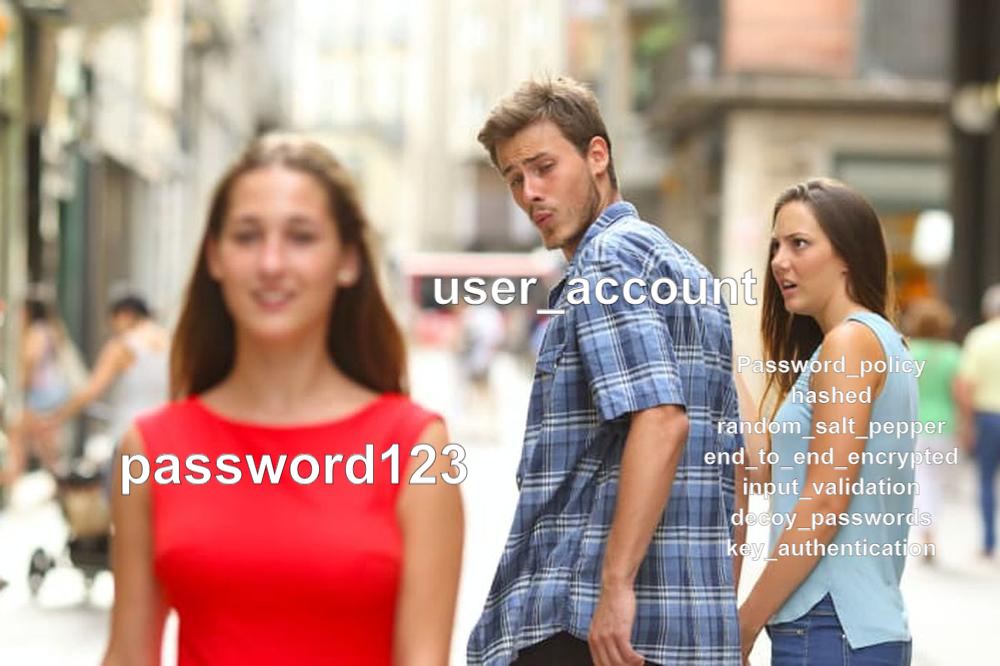
\includegraphics[width=\textwidth]{src/u8/distracted-boyfriend(3).png}

\end{enumerate}

\end{document}